\documentclass[article, 11pt]{IEEEtran}   %Document is an article, 11 pt font, and follows IEEE format
\usepackage{hyperref}         %Use hyperref package (for hyperlinks)
\usepackage{graphicx}         %Use graphicx package (for images)
\usepackage{float}            %Use float package (allows you to place images more easily)
%\usepackage{gensymb}          %Use gensymb package (generic symbols)
\usepackage{amsmath}          %Use amsmath package (for optimized math formulas)
\usepackage{tikz}             %Use tikz package (for creating graphics)
\usepackage{pgfplots}         %Use pgfplots package (for creating graphics)
\usepackage{pgfplotstable}    %Use pgfplotstable (for linear regression)
\usepackage[spanish]{babel}


\begin{document}
%
% paper title
% Titles are generally capitalized except for words such as a, an, and, as,
% at, but, by, for, in, nor, of, on, or, the, to and up, which are usually
% not capitalized unless they are the first or last word of the title.
% Linebreaks \\ can be used within to get better formatting as desired.
% Do not put math or special symbols in the title.
\title{Proyecto 1\\Aplicaciones de EDO}

% author names and affiliations
% use a multiple column layout for up to three different
% affiliations
\author{
	\IEEEauthorblockN{Juan José Rivera Román - 20002802\\Mario Esteban Ponce Contreras - 21000508}
	\IEEEauthorblockA{\\Universidad Galileo\\Guatemala, Guatemala }
}

% make the title area
\maketitle

% As a general rule, do not put math, special symbols or citations in the abstract
\begin{abstract}
Al momento de trabajar con ecuaciones diferenciales de primer orden, no siempre es posible expresar la solución de manera explícita o ímplicita, aun cuando sea posible demostrar que dicha solución existe. En esos casos, una forma de expresar la solución a una ecuacion diferencial es por medio de algún método numérico. En este proyecto se estudia y aplica el método de Runge-Kutta, uno de los métodos numéricos más precisos.
\end{abstract}

\section{Introducci\'on}
En este proyecto se pone en práctica lo aprendido en el curso de ecuaciones diferenciales ordinarias, los distintos tipos de métodos para encontrar las soluciones generales y particulares, además, se explorará el método de aproximación de Runge-Kutta que permite aproximar la solución a una ecuación diferencial de primer orden con valores iniciales $y\prime=f(x, y), y(x_o)=y_o$.

El objetivo principal del proyecto es entender y aplicar el método de aproximación de Runge-Kutta, comparar los resultados con el método analítico estudiado en clase y comprobar la presición del método para la resolución de ecuaciones diferenciales dados ciertos valores iniciales.

\section{Procedimiento}
Se inició la práctica investigando en distintas fuentes el método de Runge-Kutta, cómo utilizarlo y las condiciones que deben cumplir para aplicar el método. Luego se procedió a abstraer el método en código de programación para facilitar la realización pruebas que permitan validar el correcto funcionamiento del algoritmo aplicado. Finalmente, se diseñó e implementó una interfaz de usuario para que cualquier usuario pueda hacer uso del algoritmo sin conocimiento previo en programación.

\subsection{Materiales}
\begin{itemize}       							%Creating an unordered list
\item Computadora con Visual Studio Code y procesador de 1.80GHz mínimo.
\item Software: Nodejs, npm y Vue-cli.
\end{itemize}

\subsection{Diagrama de flujo del proyecto}

\begin{figure}[H]									%Creating a figure with caption
\centering
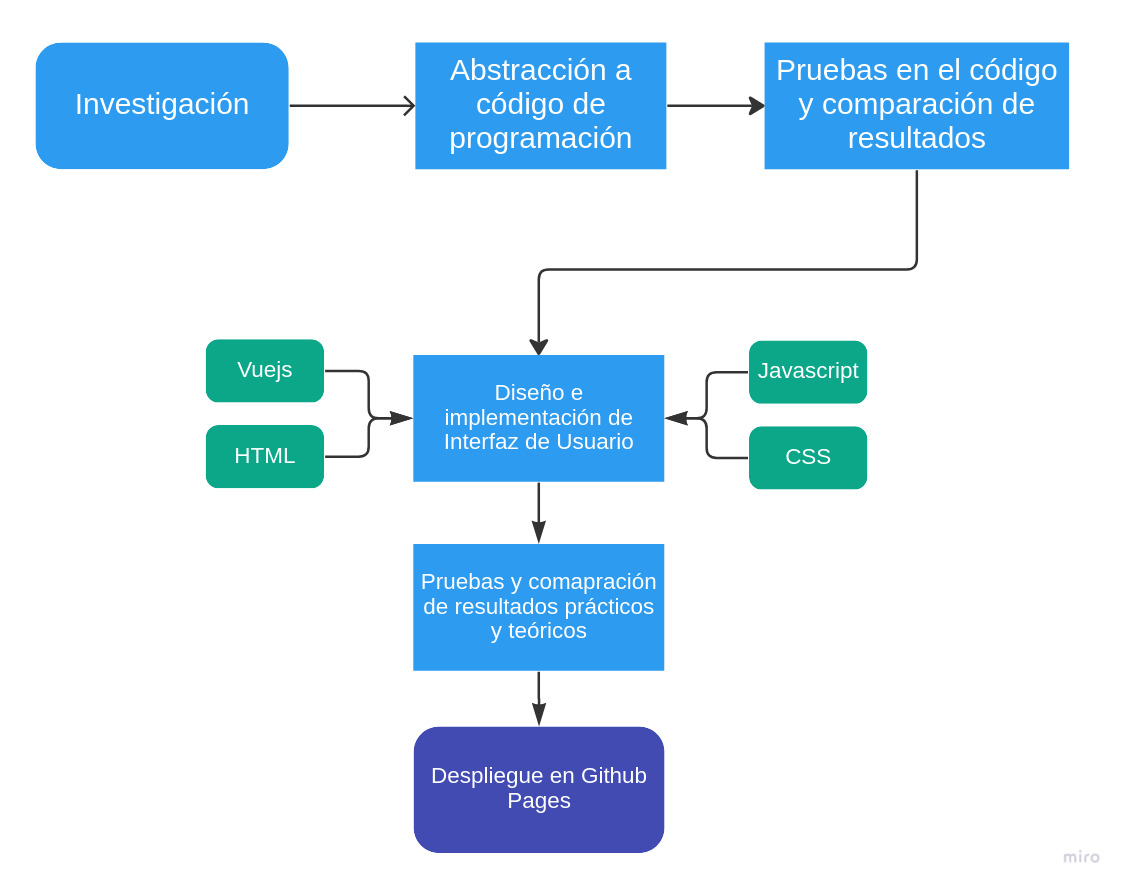
\includegraphics[scale=0.2]{flujoDeProyecto}%Inserting graphic file (in same directory)
\caption{Diagráma de flujo del proyecto}\label{diagram1}  %Captioning the graphic file
\end{figure}

\subsection{Pasos del procedimiento}        		
Siguiendo el algoritmo de aproximación del método de Runge-Kutta:
\begin{enumerate}						%Creating an ordered list
	\item Se definen la ecuación $y\prime=f(x, y)$ y sus valores iniciales $x_o$  y $y(x_o)$ además de definir el tamaño del paso $h$ entre $x_n$ y $x_{n-1}$
	\item Dependiendo del orden del método a utilizar, se calcula determinado número de términos que forman parte del promedio ponderado con el que se forma el polinomio de Taylor que se utiliza para aproximar la solución.
\end{enumerate}

\vspace{1em}

Para el métdo de primer orden:
\begin{equation}
	y_{n+1}=y_n+hf(x_n, y_n)
\end{equation}

Para el método de segundo orden:
\begin{equation}
y_{n+1}=y_n+\frac{h}{2}(k_1+k_2)
\end{equation}

Donde:
\begin{gather*}
k_1=f(x_n,y_n)\notag\\
k_2=f(x_n+h,y_n+hk_1)
\end{gather*}

Para el método de cuarto orden: 
\begin{equation}
y_{n+1}=y_n+\frac{h}{6}(k_1+2k_2+2k_3+k_4)
\end{equation}

Donde:
\begin{gather*}
k_1=f(x_n, y_n)\notag\\
k_2=f(x_n+\frac{1}{2}h, y_n+\frac{1}{2}hk_1)\\
k_3=f(x_n+\frac{1}{2}h, y_n+\frac{1}{2}hk_2)\\
k_4=f(x_n+h, y_n+hk_3)
\end{gather*}

Finalmente, se compararon los resultados obtenidos por medio del método analítico con los resultados obtenidos por medio del método de Runge-Kutta de diferente orden. En general, la aproximación es mucho mejor al aumentar el grado del método, y gráficamente, es mucho más fácil apreciar la presición del la aproximación en cuanto menor sea el paso $h$ entre cada iteración.

\section {Resultados}
\subsection{Prueba 1}
\begin{table}[H]
\centering
\caption{Datos para la prueba 1}
\label{DataTable1}
\begin{tabular}{|c|c|}
\hline
EDO & $y\prime=x+1-y$\\
Método & RK2\\
h & 0.25\\  
$y(0)$ & 0\\
x & 1\\
Solución & $y(x)=x$\\
\hline   
\end{tabular}
\end{table}

\begin{table}[H]
\centering
\caption{Resultados de la prueba 1}
\label{DataTable2}
\begin{tabular}{|c|c|c|c|c|c|}
\hline
$x_n$ & $k_1$ & $k_2$ & $y_n$ & Valor real & \% de error \\
\hline
0.00 & 0.0000 & 0.0000 & 0.0000 & 0.0000 & 0.00\%\\
0.25 & 1.0000 & 1.0000 & 0.2500 & 0.2500 & 0.00\%\\
0.50 & 1.0000 & 1.0000 & 0.5000 & 0.5000 & 0.00\%\\
0.75 & 1.0000 & 1.0000 & 0.7500 & 0.7500 & 0.00\%\\
1.00 & 1.0000 & 1.0000 & 1.0000 & 1.0000 & 0.00\%\\
\hline   
\end{tabular}
\end{table}

\begin{figure}[H]									%Creating a figure with caption
\centering
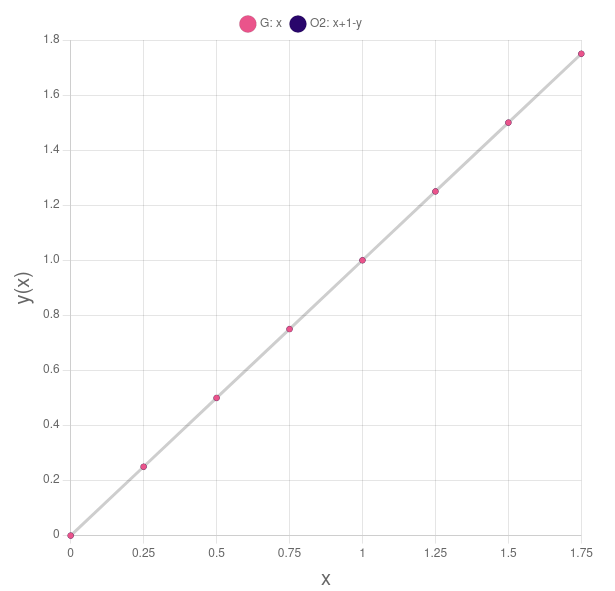
\includegraphics[scale=0.35]{graficaProblema1}%Inserting graphic file (in same directory)
\caption{Comparación gráfica de la solución analítica y la aproximación RK2}\label{diagram2}  %Captioning the graphic file
\end{figure}

\subsection{Prueba 2}
\begin{table}[H]
\centering
\caption{Datos para la prueba 2}
\label{DataTable3}
\begin{tabular}{|c|c|}
\hline
EDO & $y\prime=2y-6$\\
Método & RK4\\
h & 0.25\\  
$y(0)$ & 1\\
x & 1\\
Solución & $y(x)=3-2e^{2x}$\\
\hline   
\end{tabular}
\end{table}

\begin{table}[H]
\centering
\caption{Resultados de la prueba 2}
\label{DataTable2}
\begin{tabular}{|c|c|c|c|c|c|}
\hline
$x_n$ & $k_1$ & $k_2$ & $k_3$ & $k_4$ \\
\hline
0.00 & 0.0000 & 0.0000 & 0.0000 & 0.0000\\
0.25 & 1.0000 & 1.0000 & 0.2500 & 0.2500\\
0.50 & 1.0000 & 1.0000 & 0.5000 & 0.5000\\
0.75 & 1.0000 & 1.0000 & 0.7500 & 0.7500\\
1.00 & 1.0000 & 1.0000 & 1.0000 & 1.0000\\
\hline   
\end{tabular}
\end{table}

\begin{table}[H]
\centering
\begin{tabular}{|c|c|c|c|}
\hline
$x_n$ & $y_n$ & Valor real & \% de error \\
\hline
0.00 & 0.0000 & 0.0000 & 0.00\%\\
0.25 & 0.0000 & 0.0000 & 0.00\%\\
0.50 & 0.0000 & 0.0000 & 0.00\%\\
0.75 & 0.0000 & 0.0000 & 0.00\%\\
1.00 & 0.0000 & 0.0000 & 0.00\%\\
\hline   
\end{tabular}
\end{table}

\begin{figure}[H]									%Creating a figure with caption
\centering
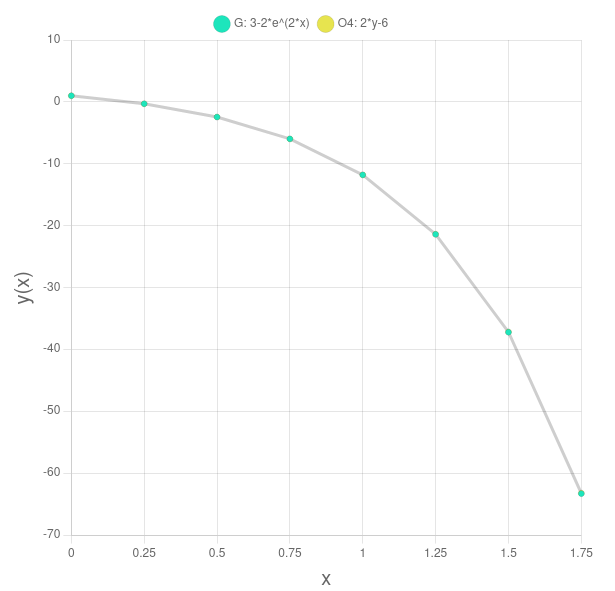
\includegraphics[scale=0.35]{graficaPrueba2}%Inserting graphic file (in same directory)
\caption{Comparación gráfica de la solución analítica y la aproximación RK4}\label{diagram2}  %Captioning the graphic file
\end{figure}

\subsection{Prueba 3}
Si la resistencia del aire es proporcional al cuadrado de la velocidad instantánea, entonces la velocidad $v$ de una masa $m$ que se deja caer desde cierta altura, con:

\begin{gather*}
m=5slugs\\
k=0.125\\
g=32\frac{pies}{s^2}
\end{gather*}

Se puede modelar como:
\begin{equation}
v\prime=g-\frac{k}{m}v^2
\end{equation}

Utilizando el método de Runge-Kutta de cuarto orden con $h=1$, se calcula la velocidad del cuerpo pasados 5 segundos:

\begin{table}[H]
\centering
\caption{Resultados de la prueba 3}
\label{DataTable3}
\begin{tabular}{|c|c|c|c|c|c|c|}
\hline
$x_n$ & $k_1$ & $k_2$ & $k_3$ & $k_4$ & $y_n$ \\
\hline
1.00 & 31.9750 & 24.7856 & 27.5158 & 11.6712 & 25.7081\\
2.00 & 15.4772 & 4.0327 & 12.7836 & -5.0406 & 33.0531\\
3.00 & 4.6872 & 0.6767 & 4.1252 & -2.5557 & 35.0090\\
4.00 & 1.3591 & 0.1580 & 1.2207 & -0.8148 & 35.5593\\
5.00 & 0.3883 & 0.0421 & 0.3508 & -0.2385 & 35.7153\\
\hline   
\end{tabular}
\end{table}

Utilizando la solución analítica:
\begin{equation}
y(x)=\frac{16\sqrt5(e^{4x/\sqrt5}-1)}{e^{4x/\sqrt5}+1}
\end{equation}
\newpage

\begin{table}[H]
\centering
\caption{Comparación de Resultados de la prueba 3}
\label{DataTable4}
\begin{tabular}{|c|c|c|c|}
\hline
$x_n$ & $y_n$ & Valor real & \% de error \\
\hline
1.00 & 25.7081 & 25.5295 & 0.70\%\\
2.00 & 33.0531 & 33.8322 & 2.30\%\\
3.00 & 35.0090 & 35.4444 & 1.23\%\\
4.00 & 35.5593 & 35.7212 & 0.45\%\\
5.00 & 35.7153 & 35.7677 & 0.15\%\\
\hline   
\end{tabular}
\end{table}

\begin{figure}[H]									%Creating a figure with caption
\centering
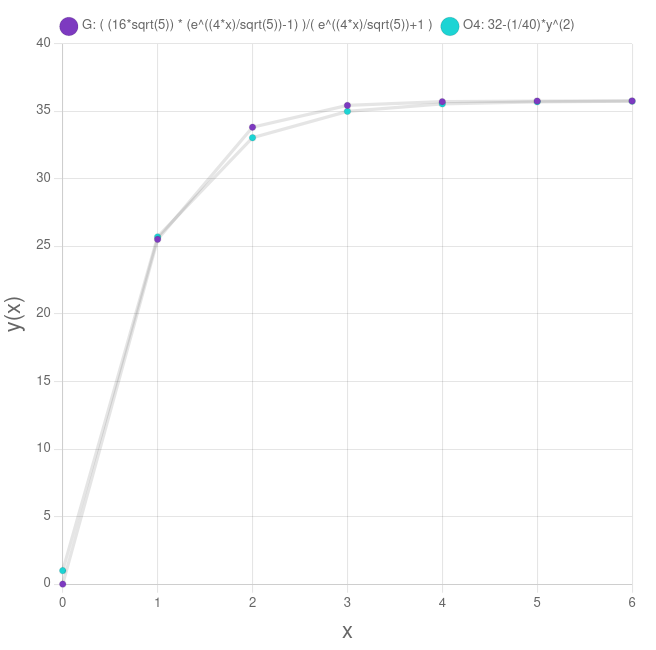
\includegraphics[scale=0.35]{graficaPrueba3}%Inserting graphic file (in same directory)
\caption{Comparación gráfica de la solución analítica y la aproximación RK4}\label{diagram4}  %Captioning the graphic file
\end{figure}

\section{Discusi\'on / An\'alisis}
Tanto en la Prueba 1 como en la Prueba 2, los valores apróximados por el método de Runge-Kutta se acercaron significativamente a los valores calculados de manera analítica, esto se hace aún más evidente al observar las gráficas, tanto la gráfica de la solución exácta como la gráfica de la aproximación por el método de Runge-Kutta se superponen, dejando en claro que sus valores son casi idénticos.
\vspace{1em}

En el caso de la prueba 2, a pesar de que el porcentaje de error fue mayor, este es aun menor al 0.2\%, lo que lo hace una aproximación lo suficientemente exácta para la mayoría de aplicaciones.
\vspace{1em}

Para la prueba 3, la diferencia entre la velocidad en $t=5s$ calculada analíticamente y el valor aproximado con el método de Runge-Kutta es significativamente pequeña, lo que confirma la utilidad del método en aplicaciones reales y especialmente para ecuaciones diferenciales con soluciones tan complejas de obtener y expresar de manera analítica como la de la prueba 3.

\section{Conclusi\'on}
Es importante ser capaces de identificar y resolver ecuaciones diferenciales, puesto que su aplicación en el mundo real es amplia. Sin embargo, que una equación diferencial tenga una o varias soluciones, no significa necesariamente que esta pueda ser expresada de forma explícita o implícita, para estos casos en donde la solución no puede expresarse de manera simple el método de aproximación de Runge-Kutta resulta muy útil. Aun si se aplica el método de primer orden, las aproximaciones son más exáctas que con otros métodos numéricos y su implementación es relativamente sencilla, especialmente si se utiliza el recurso computacional para facilitar y acelerar el calculo de todos los datos del rango que se desea.

%FORMATO APA
\begin{thebibliography}{1}

\bibitem{Trench}
Trench, William, \emph{Elementary Differential Equations}, \url{https://digitalcommons.trinity.edu/mono/8}, Trinity University, 2013.

\bibitem{Zill}
Zill, D., \emph{Ecuaciones Diferenciales con Aplicaciones de Modelado}. Cengage Learning, 11a. edición, 2018.

\end{thebibliography}

\end{document}